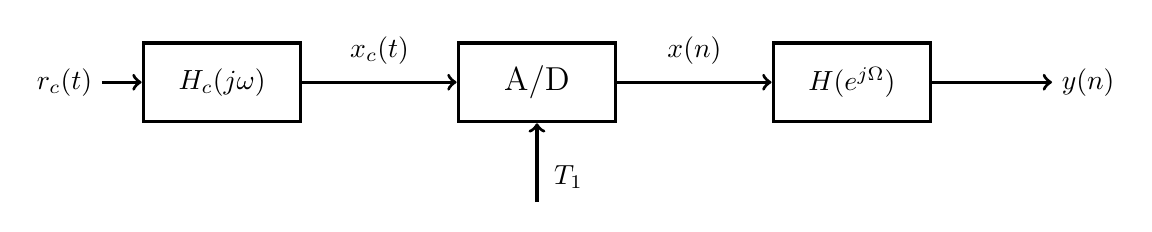
\begin{tikzpicture}[scale=1, transform shape]
    \node[rectangle, very thick, draw, minimum width=2cm, minimum height=1cm] (ad) at (0,0) {\large A/D};
    \node[rectangle, very thick, draw, minimum width=2cm, minimum height=1cm, xshift=-4cm] (hc) at (ad) {$H_c(j\omega)$};
    \node[rectangle, very thick, draw, minimum width=2cm, minimum height=1cm, xshift=4cm] (h) at (ad) {$H(e^{j\Omega})$};

    \node[xshift=-2cm] (r_c) at (hc) {$r_c(t)$};
    \node[xshift=3cm] (y_n) at (h) {$y(n)$};
    \node[xshift=-2cm,yshift=0.4cm] (x_c) at (ad) {$x_c(t)$};
    \node[xshift=2cm,yshift=0.4cm] (x_n) at (ad) {$x(n)$};
    \node[yshift=-1.2cm,xshift=0.4cm] (t1) at (ad) {$T_1$};

    \draw[->, very thick] (hc.east) -- (ad.west);
    \draw[->, very thick] (ad.east) -- (h.west);
    \draw[->, very thick] (r_c.east) -- (hc.west);
    \draw[->, very thick] (h.east) -- (y_n.west);
    \draw[->, very thick] (ad.south) ++ (0,-1cm) -- (ad.south) ;
\end{tikzpicture}